% ============================================================
% QUDA multigrid 算法实现：源码证据与可复现伪代码
% 本文件为源码快照分析报告，不覆盖同目录已有报告。
% 编译：xelatex 两遍；建议在临时输出目录中编译。
% ============================================================
\documentclass[UTF8,aspectratio=169,11pt]{ctexbeamer}

\usepackage{amsmath,amssymb}
\usepackage{booktabs}
\usepackage{tabularx}
\usepackage{array}
\usepackage{tikz}
\usetikzlibrary{arrows.meta,positioning,calc,fit,shapes.geometric}
\usepackage{xcolor}
\usepackage{microtype}
\usepackage{hyperref}

\definecolor{primary}{HTML}{17365D}
\definecolor{accent}{HTML}{1F77B4}
\definecolor{evidence}{HTML}{1E8449}
\definecolor{warning}{HTML}{C55A11}
\definecolor{muted}{HTML}{5B6573}
\definecolor{panel}{HTML}{F4F7FA}
\definecolor{violet}{HTML}{6C4A9E}
\definecolor{good}{HTML}{EAF5EE}
\definecolor{warnbg}{HTML}{FFF4E8}

\setbeamersize{text margin left=0.55cm,text margin right=0.55cm}
\setlength{\emergencystretch}{2em}
\setbeamertemplate{navigation symbols}{}
\setbeamertemplate{blocks}[rounded][shadow=false]
\setbeamercolor{normal text}{fg=black!86,bg=white}
\setbeamercolor{structure}{fg=primary}
\setbeamercolor{frametitle}{fg=primary,bg=white}
\setbeamercolor{block title}{fg=primary,bg=panel}
\setbeamercolor{block body}{fg=black!86,bg=panel}
\setbeamercolor{alerted text}{fg=warning}
\setbeamerfont{frametitle}{size=\normalsize,series=\bfseries}
\setbeamerfont{normal text}{size=\normalsize}
\setbeamertemplate{frametitle}{\vskip0.12cm\insertframetitle\par\vskip0.08cm}
\setbeamertemplate{footline}{%
  \hbox{\begin{beamercolorbox}[wd=\paperwidth,ht=2.3ex,dp=0.9ex,
    leftskip=0.55cm,rightskip=0.55cm]{author in head/foot}%
    \scriptsize\color{muted}\insertshortauthor\hfill
    \insertshorttitle\hfill\insertframenumber/\inserttotalframenumber
  \end{beamercolorbox}}}

\newcommand{\source}[1]{\vspace{0.04em}\par\noindent\parbox[t]{\linewidth}{\raggedright\tiny\color{muted}来源：#1\par}}
\newcommand{\verified}{\textcolor{evidence}{确证}}
\newcommand{\inferred}{\textcolor{accent}{推断}}
\newcommand{\unverified}{\textcolor{warning}{未验证}}
\newcommand{\codepath}[1]{\nolinkurl{#1}}

\tikzset{
  flow/.style={draw=accent,fill=accent!8,rounded corners=2pt,align=center,
    minimum height=0.68cm,text width=2.0cm,font=\scriptsize},
  state/.style={draw=primary,fill=primary!7,rounded corners=2pt,align=center,
    minimum height=0.68cm,text width=2.35cm,font=\scriptsize},
  phase/.style={draw=violet,fill=violet!8,rounded corners=2pt,align=center,
    minimum height=0.62cm,text width=2.2cm,font=\scriptsize},
  decision/.style={draw=warning,fill=warning!10,diamond,aspect=2,align=center,
    inner sep=1.5pt,font=\scriptsize},
  arrow/.style={-{Latex[length=2mm]},draw=primary,semithick},
  relation/.style={-{Latex[length=1.7mm]},draw=muted,thin,dashed}
}

\title[QUDA multigrid]{QUDA multigrid 算法实现}
\subtitle{近零模聚合、Galerkin 粗化与递归 V-cycle 的源码证据链}
\author[源码分析汇报]{源码分析汇报}
\institute{QUDA 1.1.0 参考源码快照}
\date{2026 年 8 月 28 日}

\begin{document}

\begin{frame}[plain]
  \titlepage
\end{frame}

\begin{frame}[t]{结论先行：QUDA 的 MG 是递归的自适应预条件器}
  \small
  \begin{columns}[T,totalwidth=\textwidth]
    \begin{column}{0.48\textwidth}
      \begin{block}{一条主线}
        \begin{tabular}{@{}l@{}}
          $B_\ell\;\longrightarrow\;V_\ell\;\longrightarrow\;(P_\ell,R_\ell)$ \\
          $D_{\ell+1}=R_\ell D_\ell P_\ell$ \\
          $\text{smooth}\;\longrightarrow\;\text{restrict}\;\longrightarrow\;\text{coarse solve}$ \\
          $\hspace{2.7cm}\longrightarrow\;\text{prolongate}\;\longrightarrow\;\text{smooth}$
        \end{tabular}
      \end{block}
      \begin{block}{物理/数值解释}
        平滑器快速削弱局部高频误差；由近零模张成的粗空间负责长程、低频误差。每一层重复同一逻辑，因此最底层可以是粗 Dirac 系统，而不是特殊的手写矩阵。
      \end{block}
    \end{column}
    \begin{column}{0.48\textwidth}
      \begin{block}{源码确证}
        \begin{tabular}{@{}l@{}}
          \verified\quad `MG::operator()' 实现递归 V-cycle；\\
          \verified\quad `Transfer' 同时提供 $P$ 与 $R$；\\
          \verified\quad coarse operator 由 UV/VUV 等 kernel 装配；\\
          \verified\quad `verify()' 比较 $RDP$ 与 native coarse apply。
        \end{tabular}
      \end{block}
      \begin{alertblock}{报告边界}
        以下结论来自静态源码与测试入口。\unverified\ 本次未启动 CUDA/MPI，因此不宣称具体吞吐、迭代数或硬件收敛曲线。
      \end{alertblock}
    \end{column}
  \end{columns}
  \vfill
  \begin{center}
    \begin{tikzpicture}[node distance=0.22cm and 0.25cm]
      \node[flow] (a) {细格算子\(D_0\)};
      \node[flow,right=of a] (b) {近零模\(B\)};
      \node[flow,right=of b] (c) {Transfer\(V,P,R\)};
      \node[flow,right=of c] (d) {粗算子\(D_c\)};
      \node[flow,right=of d] (e) {递归求解};
      \draw[arrow] (a)--(b)--(c)--(d)--(e);
    \end{tikzpicture}
  \end{center}
  \source{\codepath{lib/multigrid.cpp:1131-1224}；\codepath{lib/transfer.cpp}。}
\end{frame}

\begin{frame}[t]{问题的第一性原理：粗空间要近似难解的低频子空间}
  \small
  \begin{columns}[T,totalwidth=\textwidth]
    \begin{column}{0.48\textwidth}
      \begin{block}{误差分解}
        设误差为 $e=e_{\rm low}+e_{\rm high}$。局部 smoother 对 $e_{\rm high}$ 有效，但对随尺度缓慢变化的 $e_{\rm low}$ 收敛很慢。若 $V$ 的列覆盖后者，则
        \begin{equation*}
          e_{\rm low}\simeq P e_c,\qquad
          e_c\simeq (RDP)^{-1}Rr.
        \end{equation*}
      \end{block}
    \end{column}
    \begin{column}{0.48\textwidth}
      \begin{block}{维数与伴随关系}
        \begin{equation*}
          P:\mathcal V_c\to\mathcal V_f,\qquad
          R:\mathcal V_f\to\mathcal V_c,
        \end{equation*}
        聚合路径中 $R=P^\dagger$，因此
        \begin{equation*}
          D_c=RDP,\qquad P^\dagger P\simeq I_c.
        \end{equation*}
      \end{block}
      \begin{block}{量纲/实现检查}
        每个细格点必须映射到唯一粗点；每个 aggregate 内的列必须归一；粗算子 apply 必须与显式 $P\to D\to R$ 的动作相符。
      \end{block}
    \end{column}
  \end{columns}
  \vspace{0.12cm}
  \begin{center}
    \begin{tikzpicture}[node distance=0.25cm and 0.35cm]
      \node[phase] (h) {局部高频误差};
      \node[phase,right=of h] (s) {smoother\(S\)};
      \node[phase,below=of h] (l) {长程低频误差};
      \node[phase,right=of l] (c) {粗空间\(P/R\)};
      \draw[arrow] (h)--(s);
      \draw[arrow] (l)--(c);
      \draw[relation] (s)--(c);
    \end{tikzpicture}
  \end{center}
  \source{Galerkin/投影检查：\codepath{lib/multigrid.cpp:785-928}；Transfer：\codepath{include/transfer.h}。}
\end{frame}

\begin{frame}[t]{对象与生命周期：API 只负责入口，MG 层级负责状态}
  \small
  \begin{columns}[T,totalwidth=\textwidth]
    \begin{column}{0.54\textwidth}
      \begin{tabular}{@{}l@{}}
        $\text{loadGaugeQuda}(U[,C])$ \\
        $\text{mg}=\text{newMultigridQuda}(\text{mg\_param})$ \\
        $\text{invertQuda}(x,b;\;\text{preconditioner}=\text{mg})$ \\
        $\text{updateMultigridQuda}(\text{mg},\text{mg\_param})$ \\
        $\text{dumpMultigridQuda}(\text{mg},\text{mg\_param})$ \\
        $\text{destroyMultigridQuda}(\text{mg})$
      \end{tabular}
      \vspace{0.04cm}
      \begin{block}{每层运行期状态}
        \begin{tabularx}{\linewidth}{@{}lX@{}}
          \toprule
          对象 & 作用 \\
          \midrule
          $B_\ell$ & setup 生成/加载的候选近零模 \\
          $V_\ell,P_\ell,R_\ell$ & 聚合局部基与双向传输 \\
          $Y_\ell,X_\ell$ & coarse links 与 local/clover 项 \\
          smoother & pre/post 局部误差消除 \\
          coarse solver & 下一层 MG 或底层 Krylov 包装 \\
          \bottomrule
        \end{tabularx}
      \end{block}
    \end{column}
    \begin{column}{0.42\textwidth}
      \begin{block}{构造顺序}
        \begin{tikzpicture}[node distance=0.17cm]
          \node[flow,text width=2.75cm] (a) {细格 residual / smoother Dirac};
          \node[flow,text width=2.75cm,below=of a] (b) {B：随机、加载、eigensolver 或 setup};
          \node[flow,text width=2.75cm,below=of b] (c) {Transfer 与 coarse operator};
          \node[flow,text width=2.75cm,below=of c] (d) {递归下一层与 coarse solver};
          \draw[arrow] (a)--(b)--(c)--(d);
        \end{tikzpicture}
      \end{block}
      \begin{alertblock}{更新的分叉}
        thin update 复用层级结构、更新引用的 gauge/clover 与质量；full update 重新建细格 Dirac 并递归 \texttt{reset(refresh=true)}。
      \end{alertblock}
    \end{column}
  \end{columns}
  \source{API：\codepath{include/quda.h:1256-1292}；构造/更新：\codepath{lib/interface_quda.cpp:2853-3053}。}
\end{frame}

\begin{frame}[t]{层级 setup 伪代码：先建本层，再递归装配下一层}
  \small
  \begin{columns}[T,totalwidth=\textwidth]
    \begin{column}{0.64\textwidth}
      \begin{block}{语言无关等价实现}
        \footnotesize
        \begin{tabular}{@{}l@{}}
          $\text{setupLevel}(\ell,D_\ell,B_\ell,\text{cfg})$ \\
          $\quad\textbf{if }\ell<L-1:\quad B_\ell\leftarrow\text{make/load/smooth}(B_\ell)$ \\
          $\quad T_\ell\leftarrow\text{Transfer}(B_\ell,b_\mu,s_b,N_v)$ \\
          $\quad(P_\ell,R_\ell)\leftarrow T_\ell$ \\
          $\quad D_{\ell+1}\leftarrow\text{Galerkin}(D_\ell,T_\ell)$ \\
          $\quad S_\ell\leftarrow\text{makeSmoother}(D_\ell,\text{cfg}_\ell)$ \\
          $\quad B_{\ell+1}\leftarrow R_\ell B_\ell\quad(\text{或独立生成})$ \\
          $\quad MG_{\ell+1}\leftarrow\text{setupLevel}(\ell+1,D_{\ell+1},B_{\ell+1})$ \\
          $\quad C_\ell\leftarrow\text{coarseSolver}(MG_{\ell+1},S_{\ell+1})$ \\
          $\quad\textbf{return }(T_\ell,D_{\ell+1},S_\ell,C_\ell)$ \\
          $\textbf{else:}\quad S_{L-1}\leftarrow\text{bottom solver/smoother}$
        \end{tabular}
      \end{block}
    \end{column}
    \begin{column}{0.34\textwidth}
      \begin{block}{generate\_all\_levels}
        \begin{tabular}{@{}l@{}}
          TRUE：各层可独立生成 $B$；\\
          FALSE：先做 $B_{\ell+1}=R_\ell B_\ell$，\\
          再重建下一层 Transfer。\\[0.2em]
          这不是内存优化，而是改变 setup 数据流。
        \end{tabular}
      \end{block}
      \begin{alertblock}{顺序约束}
        \texttt{createCoarseDirac} 发生在 \texttt{createSmoother} 之前；下一层和 solver 在 coarse operator 建好后才创建。
      \end{alertblock}
    \end{column}
  \end{columns}
  \source{递归装配：\codepath{lib/multigrid.cpp:72-197}；伪代码为控制流等价重写。}
\end{frame}

\begin{frame}[t]{近零模 setup 伪代码：随机向量只是起点，不是最终粗空间}
  \small
  \begin{columns}[T,totalwidth=\textwidth]
    \begin{column}{0.67\textwidth}
      \begin{block}{`generateNullVectors(B,refresh)'}
        \begin{tabular}{@{}l@{}}
          $\text{maxiter}\leftarrow\text{refresh ? setup\_maxiter\_refresh : setup\_maxiter}$ \\
          $\text{solver}\leftarrow(\text{setup\_inv\_type},\text{tol},\text{precision},\text{use\_init}=\text{YES})$ \\
          $\textbf{for }q=1,\ldots,\text{num\_setup\_iter}:$ \\
          $\quad\text{可选：全局 Gram--Schmidt}(B)$ \\
          $\quad\textbf{for each batch }I\subset\{0,\ldots,N_v-1\}:$ \\
          $\qquad\textbf{if setup\_type=TEST: }(rhs,x)\leftarrow(B_I,0)$ \\
          $\qquad\textbf{else: }(rhs,x)\leftarrow(0,B_I)$ \\
          $\qquad(x\leftarrow\text{solve}(D_\ell x=rhs))$ \\
          $\qquad B_I\leftarrow x$ \\
          $\quad\text{可选：全局 Gram--Schmidt}(B)$ \\
          $\quad\textbf{if solver=MG: reset/rebuild\;T\text{，并刷新下一层}}$
        \end{tabular}
      \end{block}
    \end{column}
    \begin{column}{0.31\textwidth}
      \begin{block}{关键语义}
        `TEST' 分支以 $B$ 为右端、零初值；普通 null setup 以 $B$ 为初值、零右端，让迭代器保留慢模而衰减快模。
      \end{block}
      \begin{block}{特殊路径}
        CG/CA-CG 包装 $D^\dagger D$；MG setup 把自身作为 GCR 的预条件器；quarter halo 在 setup 期间临时提升到 half。
      \end{block}
    \end{column}
  \end{columns}
  \source{setup 参数与 batch：\codepath{lib/multigrid.cpp:1275-1413}；MG 自举：\codepath{lib/multigrid.cpp:1338-1363}；枚举：\codepath{include/enum_quda.h:464-482}。}
\end{frame}

\begin{frame}[t]{块 Gram--Schmidt：正交对象是 aggregate-local 的列，不是全局向量}
  \small
  \begin{columns}[T,totalwidth=\textwidth]
    \begin{column}{0.67\textwidth}
      \begin{block}{block orthogonalize 的数学伪代码}
        \begin{tabular}{@{}l@{}}
          $\textbf{for each aggregate }a\text{ and coarse chirality }q:$ \\
          $\quad\textbf{for }j=0,\ldots,N_v-1:\quad v_j\leftarrow B_j|_{a,q}$ \\
          $\quad\quad\textbf{for }i<j:\quad \alpha_{ij}=\sum_{x\in a}v_i(x)^\dagger v_j(x)$ \\
          $\quad\quad\quad v_j\leftarrow v_j-\alpha_{ij}v_i$ \\
          $\quad\quad n_j^2=\sum_{x\in a}\|v_j(x)\|^2$ \\
          $\quad\quad v_j\leftarrow v_j/\sqrt{n_j^2}$ \\
          $\quad\quad V_j(a,q)\leftarrow v_j$ \\
          $\textbf{repeat }n\_block\_ortho\text{ 次；two\_pass 用固定点复核/再正交}$
        \end{tabular}
      \end{block}
    \end{column}
    \begin{column}{0.31\textwidth}
      \begin{block}{实现对应}
        首轮从 $B$ 读入；后续重复轮次从 $V$ 读入。CUDA kernel 以 coarse aggregate、chirality 和向量 tile 并行化；`mVec' 只是批量化，不改变 Gram--Schmidt 顺序语义。
      \end{block}
      \begin{alertblock}{必要不变量}
        对每个 aggregate，$V_a^\dagger V_a\simeq I$。仅做全局正交不能替代这个条件。
      \end{alertblock}
    \end{column}
  \end{columns}
  \source{kernel 主循环：\codepath{include/kernels/block_orthogonalize.cuh:122-253}；精度 dispatch：\codepath{lib/block_orthogonalize.in.cu:42-308}；调用：\codepath{lib/transfer.cpp:92-112}。}
\end{frame}

\begin{frame}[t]{Transfer 伪代码：几何 map、spin map 与 $P/R$ 必须共享同一约定}
  \small
  \begin{columns}[T,totalwidth=\textwidth]
    \begin{column}{0.63\textwidth}
      \begin{block}{aggregate 路径}
        \footnotesize
        \begin{tabular}{@{}l@{}}
          $a(x)\leftarrow\text{coarseSite}(x_\mu/b_\mu)$ \\
          $s_c\leftarrow\text{spinMap}(s_f,\text{parity})$ \\
          $\textbf{P: }\psi_f(x,s_f,c_f)\leftarrow\sum_{c_c,j}V_j(x,s_f,c_f;c_c)\,\eta_c(a(x),s_c,c_c,j)$ \\
          $\textbf{R: }\eta_c(a,s_c,c_c,j)\leftarrow\sum_{x\in a,s_f,c_f}V_j(x,s_f,c_f;c_c)^\dagger\psi_f(x,s_f,c_f)$ \\
          $R=P^\dagger\quad\text{（aggregate；同一 }V,\;a(x),\;\text{spinMap）}$
        \end{tabular}
      \end{block}
    \end{column}
    \begin{column}{0.35\textwidth}
      \begin{block}{索引/边界检查}
        \texttt{fine\_to\_coarse} 覆盖每个细点；\texttt{coarse\_to\_fine} 按 aggregate 排序。block size 要整除局部格点，并受奇偶 coarse 维限制。
      \end{block}
      \begin{block}{变体}
        \begin{tabular}{@{}l@{}}
          aggregate：真正使用 $V$；\\
          coarse-KD：固定 staggered KD 结构；\\
          optimized-KD：元数据/等体积映射，\\
          不能直接套用 aggregate 公式。
        \end{tabular}
      \end{block}
    \end{column}
  \end{columns}
  \source{map/P/R：\codepath{lib/transfer.cpp:200-328}；kernel：\codepath{include/kernels/prolongator.cuh}。}
\end{frame}

\begin{frame}[t]{Galerkin 粗算子：快速 kernel 仍必须等价于 $RDP$}
  \small
  \begin{columns}[T,totalwidth=\textwidth]
    \begin{column}{0.66\textwidth}
      \begin{block}{Wilson/Clover 及其变体的装配伪代码}
        \footnotesize
        \begin{tabular}{@{}l@{}}
          $\text{exchangeGhost}(V,nFace),\qquad nFace=1\;(\text{Wilson/Clover}),\;3\;(\text{ASQTAD})$ \\
          $\textbf{if preconditioned Clover: }AV\leftarrow C^{-1}V$ \\
          $\textbf{for }\mu=0,\ldots,3\text{ and each direction}:$ \\
          $\quad UV_\mu\leftarrow U_\mu V\quad(\text{或 }U_\mu AV)$ \\
          $\quad Y_\mu\mathrel{+}=V^\dagger(UV_\mu)$ \\
          $\quad\textbf{if long link: }LV_\mu\leftarrow L_\mu V;\;Y_\mu\mathrel{+}=V^\dagger(LV_\mu)$ \\
          $\textbf{if not bidirectional: }Y_{+\mu}\leftarrow\text{reverse}(Y_{-\mu})$ \\
          $X\leftarrow V^\dagger C V+I+\text{twisted-mass/local terms}$ \\
          $\textbf{return }D_c=(X\text{ 的 local block})+(Y\text{ 的 hopping blocks})$
        \end{tabular}
      \end{block}
    \end{column}
    \begin{column}{0.32\textwidth}
      \begin{block}{为什么有 UV/VUV}
        $UV$ 先把 fine link 作用到所有基向量；$V^\dagger(UV)$ 再投影到粗颜色/自旋。这样避免逐列显式构造矩阵，且可在 kernel 中原子累加。
      \end{block}
      \begin{alertblock}{双向链接}
        普通 Wilson 可单向构造后反推；PC Clover、twisted mass、KD 等路径会强制 bidirectional build。
      \end{alertblock}
    \end{column}
  \end{columns}
  \source{粗化总流程：\codepath{lib/coarse_op.cuh:947-1463}；UV/VUV kernel：\codepath{include/kernels/coarse_op_kernel.cuh}。}
\end{frame}

\begin{frame}[t]{$X$、PC 与 coarse-on-coarse：局部项不能被“只粗化 hopping”替代}
  \small
  \begin{columns}[T,totalwidth=\textwidth]
    \begin{column}{0.48\textwidth}
      \begin{block}{local block 的装配}
        \footnotesize
        \begin{tabular}{@{}l@{}}
          $\textbf{if Clover: }X\leftarrow V^\dagger C V$ \\
          $\textbf{else: }X\leftarrow I$ \\
          $\textbf{if twisted mass: }X\leftarrow X+\mu\text{ term}$ \\
          $\textbf{if staggered: }X\leftarrow X+\text{staggered mass}$ \\
          $\textbf{if coarse-on-coarse: }C\text{ 取上一层 coarse clover}$
        \end{tabular}
      \end{block}
      \begin{block}{精度安全}
        half/fixed-point 路径先求 max 与 scale，再 atomic accumulate、convert/rescale；scale 是数值协议的一部分，不是单纯的存储细节。
      \end{block}
    \end{column}
    \begin{column}{0.48\textwidth}
      \begin{block}{预条件 coarse operator}
        \footnotesize
        \begin{tabular}{@{}l@{}}
          $D_c=\begin{pmatrix}A_e& D_{eo}\\D_{oe}&A_o\end{pmatrix}$ \\
          $\widehat D_{eo}=A_e^{-1}D_{eo},\qquad
            \widehat D_{oe}=A_o^{-1}D_{oe}$ \\
          $\text{PC smoother/solver: only one parity enters transfer}$ \\
          $\text{full solution: reconstruct the other parity}$
        \end{tabular}
      \end{block}
      \begin{alertblock}{配置合同}
        \texttt{coarse\_grid\_solution\_type=MATPC} 要求相应的 preconditioned smoother；full 与 parity 方案不能混用。
      \end{alertblock}
    \end{column}
  \end{columns}
  \vspace{0.08cm}
  \begin{center}
    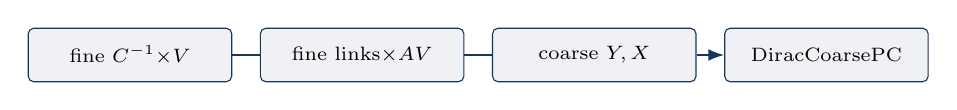
\begin{tikzpicture}[node distance=0.28cm and 0.35cm]
      \node[state] (a) {fine \(C^{-1}\)\(\times V\)};
      \node[state,right=of a] (b) {fine links\(\times AV\)};
      \node[state,right=of b] (c) {coarse \(Y,X\)};
      \node[state,right=of c] (d) {DiracCoarsePC};
      \draw[arrow] (a)--(b)--(c)--(d);
    \end{tikzpicture}
  \end{center}
  \source{local/PC：\codepath{lib/coarse_op.cuh:1345-1463}；\codepath{lib/dirac_coarse.cpp:488-656}。}
\end{frame}

\begin{frame}[t]{递归 V-cycle（1/2）：先明确 solution type 与 residual 来源}
  \small
  \begin{columns}[T,totalwidth=\textwidth]
    \begin{column}{0.67\textwidth}
      \begin{block}{进入本层的伪代码}
        \begin{tabular}{@{}l@{}}
          $\text{outerType}\leftarrow(b\text{ 是 full ? MAT : MATPC})$ \\
          $\text{innerType}\leftarrow\text{coarse\_grid\_solution\_type}_\ell$ \\
          $\text{uniform}\leftarrow(\text{smooth solve type} = \text{innerType})$ \\
          $\text{prepare}(out,in,x,b,\text{outerType})$ \\
          $\textbf{if presmoother: }(out,in)\leftarrow S_{pre}(out,in)$ \\
          $\textbf{if not uniform: }x\leftarrow\text{reconstruct}(x,b,\text{innerType})$ \\
          $\textbf{if need explicit residual: }r\leftarrow b-Dx$ \\
          $\text{residual}\leftarrow\text{solver residual / }in/ b/ r\quad\text{按分支选择}$
        \end{tabular}
      \end{block}
    \end{column}
    \begin{column}{0.31\textwidth}
      \begin{block}{为什么不能只写 $r=b-Dx$}
        预条件 smoother 可能只在单奇偶子格工作。若 solver 与 coarse solution type 不一致，必须先 reconstruct，再显式用 residual Dirac 重算 $r$。
      \end{block}
      \begin{alertblock}{非法组合}
        MATPC coarse solution 要求 preconditioned smoother；源码在运行前直接报错。
      \end{alertblock}
    \end{column}
  \end{columns}
  \source{运行期入口与 uniform/residual 分支：\codepath{lib/multigrid.cpp:1131-1183}；solution type 设定：\codepath{tests/utils/set_params.cpp:555-640}。}
\end{frame}

\begin{frame}[t]{递归 V-cycle（2/2）：限制、粗解、校正、后平滑}
  \small
  \begin{block}{按源码控制流展开}
    \begin{tabular}{@{}l@{}}
      $r_c\leftarrow R_\ell\,\text{residual}$ \\
      $e_c\leftarrow C_\ell(r_c)\quad\text{（下一层 MG 或底层 Krylov）}$ \\
      $\textbf{if no presmoother: }x\leftarrow x+P_\ell e_c$ \\
      $\textbf{else: }\delta\leftarrow P_\ell e_c;\quad x\leftarrow x+\delta$ \\
      $\textbf{if not uniform: }\text{prepare}(out,in,x,b,\text{innerType})$ \\
      $\textbf{if postsmoother: }(out,in)\leftarrow S_{post}(out,in)$ \\
      $x\leftarrow\text{reconstruct}(x,b,\text{outerType})$ \\
      $\textbf{return }x$ \\
      $\textbf{bottom level: prepare}\to\text{pre-smooth/solve}\to\text{reconstruct}$
    \end{tabular}
  \end{block}
  \begin{columns}[T,totalwidth=\textwidth]
    \begin{column}{0.48\textwidth}
      \begin{block}{残差与校正的关键}
        有 pre-smoother 时，$P e_c$ 要加到已经平滑的 $x$；源码把校正写入临时 residual，再 `xpy' 累加，避免覆盖平滑解。
      \end{block}
    \end{column}
    \begin{column}{0.48\textwidth}
      \begin{block}{数学闭环}
        \begin{equation*}
          x\xrightarrow{S_{pre}}x_s\xrightarrow{R(b-Dx_s)}e_c
          \xrightarrow{P}x_s+Pe_c\xrightarrow{S_{post}}x^+.
        \end{equation*}
      \end{block}
    \end{column}
  \end{columns}
  \source{V-cycle：\codepath{lib/multigrid.cpp:1131-1224}；coarse solver：\codepath{lib/multigrid.cpp:535-702}。}
\end{frame}

\begin{frame}[t]{coarse solver 与 cycle：V-cycle 不是唯一的“求解器对象”}
  \small
  \begin{columns}[T,totalwidth=\textwidth]
    \begin{column}{0.49\textwidth}
      \begin{block}{wrapper 语义}
        \scriptsize
        \begin{tabular}{@{}l@{}}
          $\text{coarse solver}=\text{PreconditionedSolver}(\text{solver},\text{MG/smoother})$ \\
          $\text{solver}\in\{\text{GCR},\text{CGNR/CGNE},\text{BiCGStabL},\text{CA variants},\ldots\}$ \\
          $\text{next level MG}\;\Rightarrow\;\text{one application of recursive preconditioner}$ \\
          $\text{bottom level}\;\Rightarrow\;\text{Krylov solve/deflation as configured}$
        \end{tabular}
      \end{block}
    \end{column}
    \begin{column}{0.49\textwidth}
      \begin{block}{当前快照实际支持的分支}
        \begin{tabular}{@{}l@{}}
          \texttt{QUDA\_MG\_CYCLE\_VCYCLE}：中间层可直接复用 coarse MG；\\
          \texttt{QUDA\_MG\_CYCLE\_RECURSIVE}：创建 solver wrapper；\\
          FCYCLE/WCYCLE 枚举存在，但本实现工厂未走通用分支。\\[0.2em]
          不能只凭枚举名声称已实现完整 F/W cycle。
        \end{tabular}
      \end{block}
      \begin{alertblock}{外层关系}
        MG 作为外层 Krylov 的 preconditioner 时，一次 MG 调用是 $K(r)$；粗层精度、Schwarz 和 setup 状态使其表现为可变预条件器。
      \end{alertblock}
    \end{column}
  \end{columns}
  \source{cycle/wrapper：\codepath{lib/multigrid.cpp:535-702}；枚举：\codepath{include/enum_quda.h:178-184}。}
\end{frame}

\begin{frame}[t]{实现层：halo、checkerboard、低精度与 MMA 只改变“如何算”}
  \small
  \begin{columns}[T,totalwidth=\textwidth]
    \begin{column}{0.62\textwidth}
      \begin{block}{粗算子/粗 dslash 的后端伪代码}
        \begin{tabular}{@{}l@{}}
          $\text{exchangeGhost}(V,\text{depth}=nFace)$ \\
          $\textbf{for direction }\mu:\quad\text{load local/ghost coarse spinor}$ \\
          $\quad y\leftarrow Y_\mu\,\text{spinor}_{x+\hat\mu}+Y_\mu^\dagger\,\text{spinor}_{x-\hat\mu}$ \\
          $\quad y\leftarrow y+X\,\text{spinor}_x$ \\
          $\text{bulk kernel}\parallel\text{halo kernel};\quad\text{parity/checkerboard separate}$
        \end{tabular}
      \end{block}
      \begin{block}{优化不变量}
        global/shared atomic、parity flip、coarse-color wave、autotuning、MMA/tensor-core 只替换 tile 和调度；$V^\dagger$、方向共轭转置和 $R=P^\dagger$ 不能变。
      \end{block}
    \end{column}
    \begin{column}{0.34\textwidth}
      {\scriptsize
      \begin{tabularx}{\linewidth}{@{}>{\raggedright\arraybackslash}p{0.46\linewidth}>{\raggedright\arraybackslash}X@{}}
        \toprule
        开关/字段 & 影响 \\
        \midrule
        `location' & 每层 CPU/GPU 放置 \\
        \texttt{setup\_location} & null/setup 与粗算子构造位置 \\
        \texttt{precision\_null} & $B/V$ 存储精度 \\
        \begin{tabular}{@{}l@{}}\texttt{smoother\_halo\_}\\\texttt{precision}\end{tabular} & smoother halo 精度 \\
        \begin{tabular}{@{}l@{}}\texttt{setup/dslash/}\\\texttt{transfer\_use\_mma}\end{tabular} & 三类 kernel 的 MMA 选择 \\
        fixed-point & max/scale/convert 协议 \\
        \bottomrule
      \end{tabularx}}
    \end{column}
  \end{columns}
  \source{粗算子 kernel：\codepath{lib/coarse_op.cuh:221-915}；coarse Dirac：\codepath{lib/dirac_coarse.cpp:121-479}。}
\end{frame}

\begin{frame}[t]{参数合同：最少要同步几何、零空间、solver 与 solution type}
  \small
  {\scriptsize
  \begin{tabularx}{\textwidth}{@{}>{\raggedright\arraybackslash}p{1.35cm}>{\raggedright\arraybackslash}p{4.25cm}>{\raggedright\arraybackslash}X@{}}
    \toprule
    参数组 & 代表字段 & 实现含义 \\
    \midrule
    层级/几何 & \texttt{n\_level}、\texttt{geo\_block\_size}、\texttt{spin\_block\_size} & 粗格体积、aggregate 容量、spin/chirality map；block 需满足整除和 parity 约束。 \\
    零空间 & \texttt{n\_vec}、\texttt{n\_vec\_batch}、\texttt{setup\_type} & 列数、批处理和 TEST/null setup 分支；batch 不整除直接失败。 \\
    setup & \texttt{setup\_inv\_type}、\texttt{num\_setup\_iter}、\texttt{setup\_tol} & 生成/刷新 $B$ 的迭代器、次数与停机目标。 \\
    Transfer & \texttt{transfer\_type}、\texttt{precision\_null} & aggregate、KD 或 optimized-KD；决定是否有实际 $V$。 \\
    smooth & \texttt{smoother}、\texttt{nu\_pre/post}、\texttt{omega}、Schwarz & pre/post 应用次数、松弛与局部预条件。 \\
    coarse & \texttt{coarse\_solver}、\texttt{coarse\_grid\_solution\_type} & 下一层 wrapper、底层 Krylov，以及 full/PC residual 语义。 \\
    \bottomrule
  \end{tabularx}}
  \vspace{0.12cm}
  \begin{alertblock}{一个容易漏掉的约束}
    \texttt{generate\_all\_levels=false} 且计算 null vectors 时，各层 \texttt{n\_vec} 必须一致；否则参数检查拒绝配置。\quad \texttt{MATPC} solution 又要求 preconditioned smoother。
  \end{alertblock}
  \source{参数结构/检查：\codepath{include/quda.h:638-836}；\codepath{lib/check_params.h:930-1075}。}
\end{frame}

\begin{frame}[t]{验证矩阵：把“粗化正确”拆成可定位的不变量}
  \small
  \begin{columns}[T,totalwidth=\textwidth]
    \begin{column}{0.62\textwidth}
      \begin{block}{验证伪代码}
        \begin{tabular}{@{}l@{}}
          $\textbf{for null vector }B_i:\quad e_i\leftarrow B_i-P(RB_i)$ \\
          $\textbf{for coarse random }\eta:\quad z\leftarrow\eta-R(P\eta)$ \\
          $\textbf{for coarse random }\eta:\quad
             z\leftarrow D_c\eta-R(D(P\eta))$ \\
          $\textbf{if PC: }\quad z\leftarrow \widehat D_c\eta-A_c^{-1}D_c\eta$ \\
          $\textbf{check normality: }\operatorname{Im}\langle\eta,M^\dagger M\eta\rangle\simeq0$ \\
          $\textbf{optional: }\text{low-mode overlap / oblique projection}$ \\
          $\textbf{fail if relative L2 or max deviation exceeds tolerance}$
        \end{tabular}
      \end{block}
    \end{column}
    \begin{column}{0.34\textwidth}
      \begin{tabularx}{\linewidth}{@{}lX@{}}
        \toprule
        失败项 & 优先回查 \\
        \midrule
        $PRB\neq B$ & block ortho、map、$V$ 精度 \\
        $RP\eta\neq\eta$ & $R/P$ spin/parity 与归一化 \\
        $RDP\neq D_c$ & UV/VUV、方向、local $X$ \\
        PC 误差大 & $C^{-1}V$、Schur parity、重构 \\
        normality 失败 & dagger/halo/粗 dslash \\
        \bottomrule
      \end{tabularx}
    \end{column}
  \end{columns}
  \vspace{0.08cm}
  \begin{alertblock}{源码中的诚实边界}
    ASQTAD 的三跳 long link 在 KD 或 aggregate 太小时会主动跳过部分 verify；这应记录为“验证条件不满足”，不能记成通过。
  \end{alertblock}
  \source{verify：\codepath{lib/multigrid.cpp:785-1129}；ASQTAD 条件：\codepath{lib/multigrid.cpp:883-928}。}
\end{frame}

\begin{frame}[t]{测试与动态演化：源码提供回归入口，但不替代本次运行证据}
  \small
  \begin{columns}[T,totalwidth=\textwidth]
    \begin{column}{0.49\textwidth}
      \begin{block}{\texttt{multigrid\_evolve\_test}}
        \begin{tabular}{@{}l@{}}
          $\text{set defaults}\to\text{parse MG options}\to\text{load }U,C$ \\
          $\text{mg}\leftarrow\text{newMultigridQuda}(\text{mg\_param})$ \\
          $\text{invert}(x,b)$ \\
          $\textbf{for gauge step: }U\leftarrow\text{Monte/reunitarize}$ \\
          $\quad\text{load }U,C;\;\text{updateMultigridQuda}(\text{mg})$ \\
          $\quad\text{invert}(x,b)$ \\
          $\textbf{for mass step: }(m,\kappa,\mu)\leftarrow\text{new values}$ \\
          $\quad\text{update MG}\to\text{invert}$
        \end{tabular}
      \end{block}
    \end{column}
    \begin{column}{0.49\textwidth}
      \begin{block}{\texttt{multigrid\_benchmark\_test}}
        初始化 `DiracCoarse' 与 `DiracCoarsePC'，可对 Dslash、Mat、Clover、$M^\dagger$、$M^\dagger M$ 及 PC 变体做 gflop/s 测量；还可由 gtest 检查动作。
      \end{block}
      \begin{alertblock}{本报告的验证状态}
        \verified\quad 已核对测试控制流与参数默认值。\\
        \unverified\quad 未执行编译后的 CUDA/MPI 测试，故没有把源码中的测试能力写成实测结果。
      \end{alertblock}
    \end{column}
  \end{columns}
  \source{演化测试：\codepath{tests/multigrid_evolve_test.cpp:308-452}；benchmark：\codepath{tests/multigrid_benchmark_test.cpp}。}
\end{frame}

\begin{frame}[t]{从零复现的最短路径：先做 golden reference，再开优化}
  \small
  \begin{block}{推荐的逐级实现顺序}
    \begin{tabular}{@{}l@{}}
      $\textbf{0. 约定：}\;\text{固定 lattice ordering、parity、spin/color、边界条件和质量归一化}$ \\
      $\textbf{1. 单 rank：}\;\text{随机 }B\to\text{aggregate-local GS}\to V\to(P,R)$ \\
      $\textbf{2. Golden coarse：}\;D_c\eta\equiv R\,[D\,(P\eta)]\quad\text{逐粗基/逐动作实现}$ \\
      $\textbf{3. 快速 coarse：}\;\text{替换为 UV/VUV、local }X\text{，逐动作比较 golden}$ \\
      $\textbf{4. 递归 solve：}\;\text{加入 pre/post smoother、residual 分支与 bottom solver}$ \\
      $\textbf{5. PC/MPI：}\;\text{加入 Schur prepare/reconstruct、ghost、双向 link 和 halo 精度}$ \\
      $\textbf{6. 性能：}\;\text{half/fixed-point、atomic、MMA、autotune；每步保留 verify}$
    \end{tabular}
  \end{block}
  \begin{columns}[T,totalwidth=\textwidth]
    \begin{column}{0.48\textwidth}
      \begin{block}{每次实验记录}
        lattice/global partition、\texttt{n\_vec}、block size、setup solver、smoother、cycle、solution type、各精度、verify deviation、迭代数与时间。
      \end{block}
    \end{column}
    \begin{column}{0.48\textwidth}
      \begin{alertblock}{风险排序}
        先排除数学不一致（$P/R/D_c$），再排除 checkerboard/halo，最后才讨论低精度和 kernel 性能；否则性能优化会掩盖粗化错误。
      \end{alertblock}
    \end{column}
  \end{columns}
  \source{实现依据：\codepath{lib/transfer.cpp:200-328}、\codepath{lib/coarse_op.cuh:1043-1463}、\codepath{lib/multigrid.cpp:1131-1224}。该页是面向复现的工程排序。}
\end{frame}

\begin{frame}[t]{最终结论与源码索引}
  \small
  \begin{columns}[T,totalwidth=\textwidth]
    \begin{column}{0.54\textwidth}
      \begin{block}{一句话结论}
        QUDA 的 multigrid 不是一个固定的“粗网格矩阵”：它是由 setup 产生的局部正交近零模、Galerkin coarse operator、PC/Schur 约定、递归 solver wrapper 和 GPU/MPI 数据路径共同构成的状态机。
      \end{block}
      \begin{tabular}{@{}l@{}}
        $B\;\to\;V\;\to\;RDP\;\to\;\text{recursive V-cycle}$ \\
        $\text{verify }(PRB,RP\eta,RDP\eta,\text{PC},\text{normality})$ \\
        $\text{only then enable half/fixed-point/MMA/halo optimizations}$
      \end{tabular}
    \end{column}
    \begin{column}{0.42\textwidth}
      \begin{tabularx}{\linewidth}{@{}lX@{}}
        \toprule
        主题 & 主要源码 \\
        \midrule
        层级/setup & \codepath{lib/multigrid.cpp} \\
        P/R 与 map & \codepath{lib/transfer.cpp}, \codepath{include/transfer.h} \\
        block GS & \codepath{include/kernels/block_orthogonalize.cuh} \\
        coarse operator & \codepath{lib/coarse_op.cuh} \\
        coarse Dirac/PC & \codepath{lib/dirac_coarse.cpp} \\
        API/参数/测试 & \codepath{lib/interface_quda.cpp}, \codepath{include/quda.h}, \codepath{tests/} \\
        \bottomrule
      \end{tabularx}
    \end{column}
  \end{columns}
  \vfill
  \begin{center}
    \textcolor{muted}{报告完成标准：源码控制流可追踪，伪代码可迁移，验证边界已显式标注。}
  \end{center}
  \source{综合依据：\codepath{lib/multigrid.cpp}；\codepath{lib/transfer.cpp}；\codepath{lib/coarse_op.cuh}。}
\end{frame}

\end{document}
